% Document class and parameters %
\documentclass[10pt,a4paper]{article}

% Document packages %
\usepackage{graphicx}
\usepackage{biblatex}
\usepackage{parskip}
\usepackage{listings}
\usepackage{caption}
\usepackage{subcaption}
\usepackage{amsmath}
\usepackage[most]{tcolorbox}


\graphicspath{{./Images/}}
\setlength{\parskip}{1em}

% Document Body %
\begin{document}
\begin{titlepage}
	\centering
	{\scshape\LARGE Imperial College London \par}
	\vspace{1cm}
	{\scshape\Large Mathematics: Year 2\par}
	\vspace{1.5cm}
	{\huge\bfseries Systems and Component Reliability \par}
	\vspace{2cm}
	{\Large\ Xin Wang }
	\vfill
	{\large \today\par}
\end{titlepage}

\begin{abstract}
Engineering systems will inevitably fail and is deeply studied in systems engineering.  

Reliability engineering is a sub-discipline of systems engineering that studies the ability
of equipment to function without failure. 

\end{abstract}

\tableofcontents
\pagebreak

%%%%%%%%%%%%%%%%%%%%%%%%%%%%%%%%%%%%%%%%%%%%%%%%%%%%%%%%%%%%%%%%%%%%%%%%%%%%%%%%%%%%%%%%%%%%%%%%%%%%%%%%%%
% Sections Body %
\section{Introduction}

Engineering systems are basically systems of components that are combined such that the entire system
only works if the component work together in a certain specific way. Common examples are
computer networks, car engines and the human body.

It is very common to represent the system as a \textbf{circuit} i.e. a functional system that has a path
from $-$ to $+$. The most famous example is the electric circuit representing how a electrical
system is channeled in order to achieve functionality. \par
\begin{figure} [h!]
    \centering
    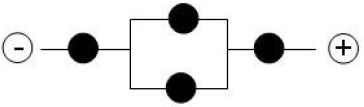
\includegraphics[scale=0.6]{circuit.JPG}
    \caption{A graphical representation of a \textbf{circuit}}
\end{figure}
Just like electrical systems, there are different types of systems that can be represented with
circuits. Every systems can be classified as series, parallel or a combination of both.

%%%%%%%%%%%%%%%%%%%%%%%%%%%%%%%%%%%%%%%%%%%%%%%%%%%%%%%%%%%%%%%%%%%%%%%%%%%%%%%%%%%%%%%%%%%%%%%%%%%%%%%%%%
\subsection{Series}

\begin{tcolorbox}[breakable,colback=white]
\textbf{Series system}: A system consisting of $n$ identical components $C_i$ in series.
\end{tcolorbox}
\begin{figure} [h!]
    \centering
    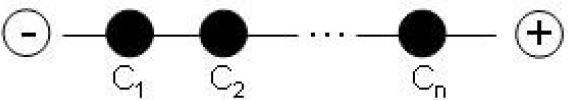
\includegraphics[scale=0.4]{serial_circuit.JPG}
\end{figure}
The failure of \textbf{any} components means that \textbf{the whole system} fails. 

If the components are \textbf{independent}, the system failure can be modelled as a probability
defined as $\Theta$.

Let $P(C_i)$ be the probability that component $C_i$ fails for $i=1,2,3,\dots,n$.
\begin{itemize}
    \item Probability that component fails: 
    $$
        P(C_i) = \Theta
    $$
    \item Probability that component \textbf{does not} fail: 
    $$
        P(\overline{C_i})=1-\Theta
    $$
    \item Probability that the system functions:
    \begin{align*}
        P(\text{Functional System}) &= P(\overline{C_1} \cap \overline{C_2} \cap \dots \cap \overline{C_n}) \\
        &= P(\overline{C_1}) \times P(\overline{C_2}) \times \dots \times P(\overline{C_n}) \\
        &= (1-\Theta)^n
    \end{align*}
\end{itemize}

\textbf{Example 1}: Given a \textbf{series system} with $n=3$ and $\Theta=0.1$, what are the
probability that the system functions?
\begin{align*}
    P(\text{Functional System}) &= (1-0.1)^3 \\
    &= (0.9)^3 \\
    &= 0.729
\end{align*}

%%%%%%%%%%%%%%%%%%%%%%%%%%%%%%%%%%%%%%%%%%%%%%%%%%%%%%%%%%%%%%%%%%%%%%%%%%%%%%%%%%%%%%%%%%%%%%%%%%%%%%%%%%
\subsection{Parallel}

\begin{tcolorbox}[breakable,colback=white]
    \textbf{Parallel system}: A system consisting of $n$ identical components $C_i$ in parallel.
\end{tcolorbox}

\begin{figure} [h!]
    \centering
    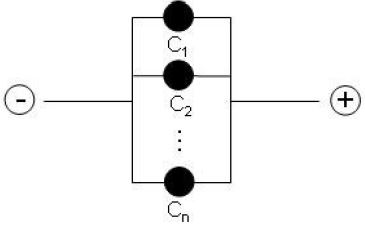
\includegraphics[scale=0.6]{parallel_circuit.JPG}
\end{figure}

The system only fails if \textbf{all} $n$ components fail. 

If the components are \textbf{independent}, the system failure can be modelled as a probability
defined as $\Theta$.

\begin{itemize}
    \item All the $n$ components have the \textbf{same} probability of failure:
    $$
        P(C_i) = \Theta
    $$
    \item Probability that the system functions:
    \begin{align*}
        P(\text{Functional System}) &= 1 - P(\text{System Failure}) \\
        &= 1 - P(C_1 \cap C_2 \cap \dots \cap C_n) \\
        &= 1 - [P(C_1) \times P(C_2) \times \dots \times P(C_n)] \\
        &= 1 - \Theta^n
    \end{align*}
\end{itemize}

\textbf{Example 2}: Given a \textbf{parallel system} with $n=3$ and $\Theta=0.1$, what are the
probability that the system functions?
\begin{align*}
    P(\text{Functional System}) &= 1 - (0.1)^3 \\
    &= 0.999
\end{align*}

%%%%%%%%%%%%%%%%%%%%%%%%%%%%%%%%%%%%%%%%%%%%%%%%%%%%%%%%%%%%%%%%%%%%%%%%%%%%%%%%%%%%%%%%%%%%%%%%%%%%%%%%%%
\pagebreak
%%%%%%%%%%%%%%%%%%%%%%%%%%%%%%%%%%%%%%%%%%%%%%%%%%%%%%%%%%%%%%%%%%%%%%%%%%%%%%%%%%%%%%%%%%%%%%%%%%%%%%%%%%
\subsection{Mixed}

Mixed systems are more complicated cases that must first be decomposed into series and parallel
systems.

For example the following circuit \par
\begin{figure}[h]
    \centering
    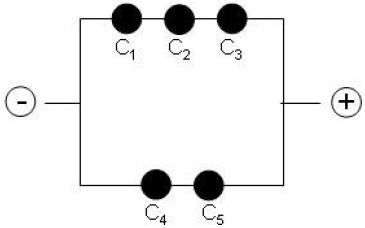
\includegraphics[scale=0.5]{mixed_circuit.JPG}
\end{figure}
can be simplified by grouping series $C_i$ together into one large abstract component
$S_n$ 

\begin{figure} [h!]
    \centering
    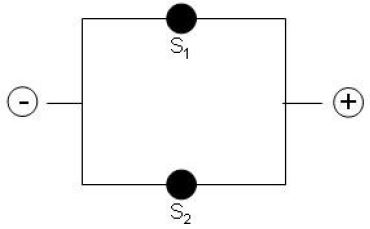
\includegraphics[scale=0.5]{mixed_circuit2.JPG}
\end{figure}

Probability that system functions:
\begin{align*}
    P(\text{Functional System}) &= 1 - P(\text{System Failure}) \\
    &= 1 - [P(S_1)\times P(S_2)\times \dots\times P(S_n)]
\end{align*}

\pagebreak

%%%%%%%%%%%%%%%%%%%%%%%%%%%%%%%%%%%%%%%%%%%%%%%%%%%%%%%%%%%%%%%%%%%%%%%%%%%%%%%%%%%%%%%%%%%%%%%%%%%%%%%%%%
\section{Time-to-failure distributions}

In engineering systems, the \textbf{random time to failure} variable $T$ is a important value.

\begin{tcolorbox}[breakable,colback=white]
\textbf{Failure rate} ($\lambda$): The frequency with which an engineered system or component fails,
expressed in failures per unit of time.
\\
\\
\textbf{Reliability rate} or \textbf{Survival rate} ($R(t)$): The probability that there is no
failure before time $t$ $(0,t]$.
$$
    R(t) = 1 - F(t)
$$
\end{tcolorbox}

A continuous failure rate means the existence of a \textbf{failure distribution} $F(t)$.

\begin{tcolorbox}[breakable,colback=white]
\textbf{Failure time distribution} ($F(t)$): A cumulative distribution function that describes the
probability of failure \textbf{up to and including time} $t$:
$$
    P(T \leq t) = F(t) = 1 - R(t)
$$
\end{tcolorbox}

The random variable $T$ is non-negative and has the following failure time distribution function:
$$
    F_T(t) = P(T \leq t)
$$
and is equal to the integral of the \textbf{failure time density}:
$$
    F_T(t) = P(T\leq t) = \int_0^t f_T (t)\: dt
$$
or alternatively:
$$
    f_T (t) = \frac{dF_T (t)}{dt} = - \frac{dR_T(t)}{dt}
$$

A common problem investigated is the probability of failure as the unit gets older i.e. finding the
probability that the unit will fail in a short interval $(t+\delta t]$ \textbf{given that it
has survived to time} $t$:
$$
    f_T(t)\delta t \approx P(t<T\leq t+\delta t)
$$
\textbf{Probability of imminent failure at time $t$}: 
$$
    P(A|B) \approx \frac{f_T(t)\delta(t)}{R_T(t)}
$$
\begin{itemize}
    \item $P(A|B)$: Probability that event $A$ occurs \textbf{given that} event $B$ occurred.
    \item $A$: The event: "\textit{unit fails in $(t+\delta t]$}" defined as $\{t<T\leq t+\delta t\}$
    \item $B$: The event: "\textit{unit not failed by time $t$}" defined as $\{T>t\}$
\end{itemize}

\begin{tcolorbox}[breakable,colback=white]
    \textbf{Hazard rate} $z_T(t)$: The likelihood of the failure of the unit after a certain time $t$ has passed.
    $$
        z_T(t) = \frac{f_T(t)}{R_T(t)} \propto P(A|B)
    $$
    where $\propto$ defined as \textit{proportional}
\end{tcolorbox}

The \textbf{cumulative hazard function} is defined as:
$$
    H_T(t) = \int_0^t z_T(u)\: du 
$$
this is related to the reliability function:
$$
    R_T(t) = e^{-H_T(t)}
$$


Summary of the symbols used:
\begin{itemize}
    \item $F$ - Failure time distribution
    \item $f$ - Failure time density 
    \item $R$ - Reliability function
    \item $z$ - Hazard rate function 
    \item $H$ - Cumulative hazard function
\end{itemize}


\textbf{Example 1}: Given $z_T(t) = \lambda$, find the following:
\begin{enumerate}
    \item Cumulative hazard:
    \begin{align*}
        H_T(t) &= \int_0^t \lambda \: du \\
        &= \lambda t
    \end{align*}
    \item Reliability function:
    \begin{align*}
        R_T(t) &= e^{-H_T(t)} \\
        &= e^{-\lambda t} 
    \end{align*}
    \item Failure density:
    \begin{align*}
        f_T(t) &= \frac{-dR_T(t)}{dt} \\
        &= \lambda e^{-\lambda t}
    \end{align*}
\end{enumerate}

\pagebreak

%%%%%%%%%%%%%%%%%%%%%%%%%%%%%%%%%%%%%%%%%%%%%%%%%%%%%%%%%%%%%%%%%%%%%%%%%%%%%%%%%%%%%%%%%%%%%%%%%%%%%%%%%%
\subsection{Hazard rate functions}

Knowledge about an item’s hazard rate often helps determine the appropriate failure time distribution for the item.

\begin{enumerate}
    \item Constant Hazard:
    $$
        z_T(t) = \lambda
    $$
    Proneness to failure at any time is \textbf{constant} and not related to time. For example,
    components that do not age like semiconductors.

    \item Increasing Hazard: 
    $$
        z_T(t) = \text{Increasing function of }t
    $$
    Item $T$ has an increasing failure rate as time $t$ increases. For example, items that age like
    charging cables.

    \item Decreasing Hazard:
    $$
        z_T(t) = \text{Decreasing function of }t
    $$
    Item $T$ has an a decreasing failure rate as time $t$ increases. For example, items manufactured
   in a factory whose process gradually improve over time.

    \item Bathtub Hazard:
    
    Name derived from the shape of the hazard function. For example, the mortality distribution of
    humans i.e. high infant mortality, a period of stabilisation then higher mortality rate due to aging.    
\end{enumerate}

\pagebreak

%%%%%%%%%%%%%%%%%%%%%%%%%%%%%%%%%%%%%%%%%%%%%%%%%%%%%%%%%%%%%%%%%%%%%%%%%%%%%%%%%%%%%%%%%%%%%%%%%%%%%%%%%%
\subsection{Life distributions}
%%%%%%%%%%%%%%%%%%%%%%%%%%%%%%%%%%%%%%%%%%%%%%%%%%%%%%%%%%%%%%%%%%%%%%%%%%%%%%%%%%%%%%%%%%%%%%%%%%%%%%%%%%
\subsubsection{Exponential distribution}

A lifetime statistical distribution that assumes a constant failure rate for the product being
modeled. 

The \textbf{1-parameter} exponential PDF is obtained by setting $\gamma=0$, and is given by: 
\begin{align*}
    f(t)=\lambda e^{-\lambda t} = \frac{1}{m}e^{\frac{1}{m}t}
\end{align*}

The \textbf{2-parameter} exponential PDF is given by: 
\begin{align*}
    f(t) = \lambda e^{-\lambda(t-\gamma} \; \text{ where } f(t)\geq 0 \text{, } \lambda>0 \text{ and } t\geq \gamma
\end{align*}

Covered previously, concluded that PDF leads to a constant hazard function as seen.
\begin{figure} [h!]
    \centering
    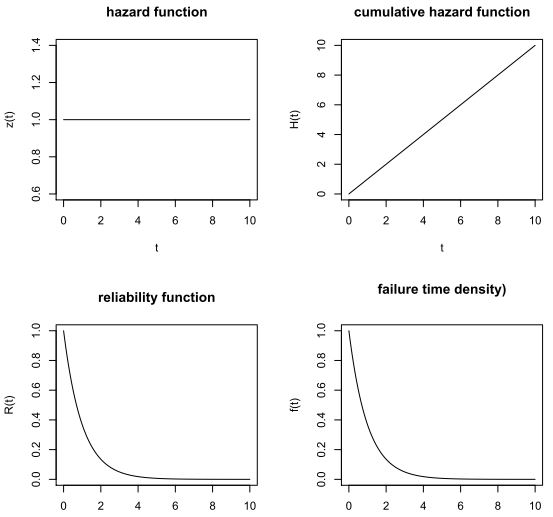
\includegraphics[scale=0.7]{exphazard.JPG}
\end{figure}

\pagebreak

%%%%%%%%%%%%%%%%%%%%%%%%%%%%%%%%%%%%%%%%%%%%%%%%%%%%%%%%%%%%%%%%%%%%%%%%%%%%%%%%%%%%%%%%%%%%%%%%%%%%%%%%%%
\subsubsection{Weibull distribution}

A statistical distribution frequently used in life data analysis. Developed by Swedish mathematician
Waloddi Weibull, this distribution is widely used due to its versatility and the fact that the
Weibull pdf can assume different shapes based on the parameter values.

The \textbf{2-parameter} Weibull PDF is obtained by setting $\gamma=0$, and is given by: 
\begin{align*}
    f(t) = \frac{C}{\eta}\left(\frac{t}{\eta}\right)^{\beta - 1}e^{{-\left(\frac{t}{\eta}\right)}^{\beta}}
\end{align*}

\begin{figure} [h!]
    \centering
    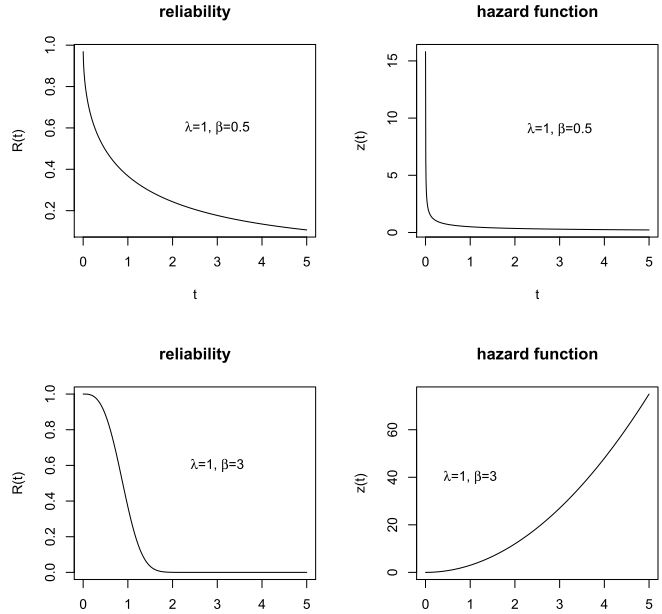
\includegraphics[scale=0.7]{weibull.JPG}
\end{figure}

The hazard function is defined as:
\begin{align*}
    z_T(t;\: \lambda, \: \beta) = \lambda \beta (\lambda t)^{\beta -1}
\end{align*}

The cumulative function is defined as:
\begin{align*}
    H_T(t;\: \lambda, \: \beta) = (\lambda t)^\beta
\end{align*}

\pagebreak

\textbf{Example 1}: A certain component has a Weibull Failure Density where $\beta = 2$ and $\lambda
= 10^{-3}$. What is the probability that a component survives longer than $500$ hours?
\begin{enumerate}
    \item List the equation to be used: 
    \begin{align*}
        R_T(t;\: \lambda, \: \beta) = 1 - F_T(t;\: \lambda, \: \beta) = e^{-(\lambda t)^\beta}
    \end{align*}
    \item Substitute values in.
    \begin{align*}
        R_T(500; \lambda = 10^{-3}, \beta = 2) &= e^{-(10^{-3}(500))^2} \\
        &= e^{-\left(\frac{1}{2}\right)^2} \\
        &= e^{-\frac{1}{4}} \\
        &\approx 0.7788 
    \end{align*}
\end{enumerate}



\pagebreak
%%%%%%%%%%%%%%%%%%%%%%%%%%%%%%%%%%%%%%%%%%%%%%%%%%%%%%%%%%%%%%%%%%%%%%%%%%%%%%%%%%%%%%%%%%%%%%%%%%%%%%%%%%
\subsection{Mean time to failure}

The value of Mean Time To Failure (MTTF) is obtained directly from the integral of $R_T(t)$ and,
thus, is defined as:
\begin{align*}
    MTTF = E[T] = \int_0^\infty tf_T(t)\: dt = -[tR_T(t)])0^\infty + \int_0^\infty R_T(t)\: dt
\end{align*}
Proof:
Since $f_T(t) = -R_T^\prime (t)$
\begin{align*}
    MTTF &= -\int_0^\infty rR_T^\prime(t) \: dt \\
    &= -[tR_T(t)])0^\infty + \int_0^\infty R_T(t)\: dt
\end{align*}

\textbf{Example 1}: Find the MTTF of the exponential distribution: $f_T(t) = \lambda e^{-\lambda t}$
\begin{align*}
    MTTF &= \int_0^\infty R_T(t) \: dt \\
    &= int_0^\infty e^{-\lambda t} \: dt \\
    &= \left[\frac{e^{\lambda t}}{-\lambda}\right]_0^\infty \\
    &= \left(0 - \frac{1}{-\lambda}\right) \\
    &= \frac{1}{\lambda}
\end{align*}

%%%%%%%%%%%%%%%%%%%%%%%%%%%%%%%%%%%%%%%%%%%%%%%%%%%%%%%%%%%%%%%%%%%%%%%%%%%%%%%%%%%%%%%%%%%%%%%%%%%%%%%%%%
\end{document} 